\documentclass[11pt,a4paper]{article}
\usepackage{amsmath}
\usepackage{enumitem}
\usepackage{fullpage}
\usepackage{graphicx}
\usepackage{pgfplots}

\begin{document}

\newcommand{\argmax}[1]{\operatorname*{arg\,max}_{#1}}

\title{COMP4680: Advanced Topics in Statistical Machine Learning\\Third Programming Assignment}
\author{Manab Chetia (u5492350), Libo Yin (u5483742)\\The Australian National University}
\maketitle

\section{Conditional Random Field Modeling}

\begin{enumerate}[label=(\alph*)]
\item
First consider a single data point $\langle D,\vec{y}\,\rangle\in D.$ By definition:
\[P(\vec{y}\,|X)=\frac{1}{Z(X)}\exp\left\{\sum_{j=1}^m\langle w_{\vec{y}_j},X_j\rangle+\sum_{j=1}^{m-1}T_{\vec{y}_j,\vec{y}_{j+1}}\right\}\]

where
\[Z(X)=\sum_{\hat{y}\in y^m}\exp\left\{\sum_{j=1}^m\langle w_{\hat{y}_j},X_j\rangle+\sum_{j=1}^{m-1}T_{\hat{y}_j,\hat{y}_{j+1}}\right\}\]

So the logarithm is:
\[\log P(\vec{y}\,|X)=\sum_{j=1}^m\langle w_{\vec{y}_j},X_j\rangle+\sum_{j=1}^{m-1}T_{\vec{y}_j,\vec{y}_{j+1}}-\log\sum_{\hat{y}\in y^m}\exp\left\{\sum_{j=1}^m\langle w_{\hat{y}_j},X_j\rangle+\sum_{j=1}^{m-1}T_{\hat{y}_j,\hat{y}_{j+1}}\right\}\]

So the gradient is:
\begin{align*}
\nabla_{w_Y}\log P(\vec{y}\,|X)&=\nabla_{w_Y}\sum_{j=1}^m\langle w_{\vec{y}_j},X_j\rangle-\frac{1}{Z(X)}\nabla_{w_Y}\sum_{\hat{y}\in y^m}\exp\left\{\sum_{j=1}^m\langle w_{\hat{y}_j},X_j\rangle+\sum_{j=1}^{m-1}T_{\hat{y}_j,\hat{y}_{j+1}}\right\}\\
&=\sum_{j=1}^m I[Y=\vec{y}_j]\vec{x}_j-\frac{1}{Z(X)}\sum_{\hat{y}\in y^m}\nabla_{w_Y}\exp\left\{\sum_{j=1}^m\langle w_{\hat{y}_j},X_j\rangle+\sum_{j=1}^{m-1}T_{\hat{y}_j,\hat{y}_{j+1}}\right\}
\end{align*}

where $Y$ is a random variable, and
\begin{align*}
\nabla_{w_Y}\exp\left\{\sum_{j=1}^m\langle w_{\hat{y}_j},X_j\rangle+\sum_{j=1}^{m-1}T_{\hat{y}_j,\hat{y}_{j+1}}\right\}&=\exp\left\{\sum_{j=1}^m\langle w_{\hat{y}_j},X_j\rangle+\sum_{j=1}^{m-1}T_{\hat{y}_j,\hat{y}_{j+1}}\right\}\nabla_{w_Y}\sum_{j=1}^m\langle w_{\hat{y}_j},X_j\rangle\\
&=\exp\left\{\sum_{j=1}^m\langle w_{\hat{y}_j},X_j\rangle+\sum_{j=1}^{m-1}T_{\hat{y}_j,\hat{y}_{j+1}}\right\}\sum_{j=1}^m I[Y=\hat{y}_j]X_j
\end{align*}

Therefore:
\begin{align*}
&\quad\nabla_{w_Y}\log P(\vec{y}\,|X)\\
&=\sum_{j=1}^m I[Y=\vec{y}_j]X_j-\frac{1}{Z(X)}\sum_{\hat{y}\in y^m}\exp\left\{\sum_{j=1}^m\langle w_{\hat{y}_j},X_j\rangle+\sum_{j=1}^{m-1}T_{\hat{y}_j,\hat{y}_{j+1}}\right\}\sum_{j=1}^m I[Y=\hat{y}_j]X_j\\
&=\sum_{j=1}^m I[Y=\vec{y}_j]X_j-\sum_{\hat{y}\in y^m}P(\hat{y}|X)\sum_{j=1}^m I[Y=\hat{y}_j]X_j\\
&=\sum_{j=1}^m I[Y=\vec{y}_j]X_j-E_{\hat{y}|X}\left[\sum_{j=1}^m I[Y=\hat{y}_j]X_j\right]
\end{align*}

Similarly:
\begin{align*}
&\quad\nabla_T\log P(\vec{y}\,|X)\\
&=\nabla_T\sum_{j=1}^{m-1}T_{\vec{y}_j,\vec{y}_{j+1}}-\nabla_T\log\sum_{\hat{y}\in y^m}\exp\left\{\sum_{j=1}^m\langle w_{\hat{y}_j},X_j\rangle+\sum_{j=1}^{m-1}T_{\hat{y}_j,\hat{y}_{j+1}}\right\}\\
&=[I(\langle i,j\rangle\in\vec{y})]_{\langle i,j\rangle \in 26\times 26}-\frac{1}{Z(X)}\sum_{\hat{y}\in y^m}\nabla_T\exp\left\{\sum_{j=1}^m\langle w_{\hat{y}_j},X_j\rangle+\sum_{j=1}^{m-1}T_{\hat{y}_j,\hat{y}_{j+1}}\right\}\\
&=[I(\langle i,j\rangle\in\vec{y})]_{\langle i,j\rangle \in 26\times 26}-\frac{1}{Z(X)}\sum_{\hat{y}\in y^m}\exp\left\{\sum_{j=1}^m\langle w_{\hat{y}_j},X_j\rangle+\sum_{j=1}^{m-1}T_{\hat{y}_j,\hat{y}_{j+1}}\right\}\nabla_T\sum_{j=1}^{m-1}T_{\hat{y}_j,\hat{y}_{j+1}}\\
&=[I(\langle i,j\rangle\in\vec{y})]_{\langle i,j\rangle \in 26\times 26}-\sum_{\hat{y}\in y^m}P(\hat{y}|X)[I(\langle i,j\rangle\in\hat{y})]_{\langle i,j\rangle \in 26\times 26}\\
&=[I(\langle i,j\rangle\in\vec{y})]_{\langle i,j\rangle \in 26\times 26}-E_{\hat{y}|X}[I(\langle i,j\rangle\in\hat{y})]_{\langle i,j\rangle \in 26\times 26}
\end{align*}

where $[I(\langle i,j\rangle\in\vec{y}\,)]_{\langle i,j\rangle \in 26\times 26}$ denotes a $26\times 26$ matrix whose value on coordinate $\langle i,j\rangle$ is 1 if $\vec{y}$ contains transition $\langle i,j\rangle$,and 0 otherwise. The above derivations naturally extend to all data points:
\begin{align*}
&\quad\log\prod_{\langle\vec{x},\vec{y}\,\rangle\in D}P(\vec{y}\,|\vec{x})=\sum_{\langle\vec{x},\vec{y}\,\rangle\in D}\log P(\vec{y}\,|\vec{x})\\
&=\sum_{\langle\vec{x},\vec{y}\,\rangle\in D}\left[\sum_{j=1}^m\langle w_{\vec{y}_j},\vec{x}_j\rangle+\sum_{j=1}^{m-1}T_{\vec{y}_j,\vec{y}_{j+1}}-\log\sum_{\hat{y}\in y^m}\exp\left(\sum_{j=1}^m\langle w_{\hat{y}_j},\vec{x}_j\rangle+\sum_{j=1}^{m-1}T_{\hat{y}_j,\hat{y}_{j+1}}\right)\right]
\end{align*}

\begin{align*}
\nabla_{w_Y}\log\prod_{\langle\vec{x},\vec{y}\,\rangle\in D}P(\vec{y}\,|\vec{x})&=\nabla_{w_Y}\sum_{\langle\vec{x},\vec{y}\,\rangle\in D}\log P(\vec{y}\,|\vec{x})\\
&=\sum_{\langle\vec{x},\vec{y}\,\rangle\in D}\nabla_{w_Y}\log P(\vec{y}\,|\vec{x})\\
&=\sum_{\langle\vec{x},\vec{y}\,\rangle\in D}\sum_{j=1}^m I(Y=\vec{y}_j)\vec{x}_j-E_{\hat{y}|\vec{x}}\left[\sum_{j=1}^m I(Y=\hat{y}_j)\vec{x}_j\right]
\end{align*}

\begin{align*}
\nabla_T\log\prod_{\langle\vec{x},\vec{y}\,\rangle\in D}P(\vec{y}\,|\vec{x})&=\nabla_T\sum_{\langle\vec{x},\vec{y}\,\rangle\in D}\log P(\vec{y}\,|\vec{x})\\
&=\sum_{\langle\vec{x},\vec{y}\,\rangle\in D}\nabla_T\log P(\vec{y}\,|\vec{x})\\
&=\sum_{\langle\vec{x},\vec{y}\,\rangle\in D}[I(\langle i,j\rangle\in\vec{y})]_{\langle i,j\rangle \in 26\times 26}-E_{\hat{y}|\vec{x}}[I(\langle i,j\rangle\in\hat{y})]_{\langle i,j\rangle \in 26\times 26}
\end{align*}

\item
From the derivations above, we can see that the features are:
\[\sum_{j=1}^m I(Y=y_j)\vec{x}_j\text{ and }[I(\langle i,j\rangle\in y)]_{\langle i,j\rangle \in 26\times 26}\]

\item
The decoder uses the max-sum algorithm. The code is located at \texttt{CRF/Decoder.py}, and the result is located at \texttt{result/decode\_output.txt}. The recursive relation of the algorithm is shown as follows:
\begin{align*}
\argmax{\vec{y}}P(\vec{y}\,|\vec{x})&=\argmax{\vec{y}}\frac{1}{Z(\vec{x})}\exp\left(\sum_{j=1}^m\langle w_{\vec{y}_j},\vec{x}_j\rangle+\sum_{j=1}^{m-1}T_{\vec{y}_j,\vec{y}_{j+1}}\right)\\
&\quad\text{since }Z(\vec{x})\text{ is a constant, and the exponential function is monotonic}\\
&=\argmax{\vec{y}}\left(\sum_{j=1}^m\langle w_{\vec{y}_j},\vec{x}_j\rangle+\sum_{j=2}^m T_{\vec{y}_{j-1},\vec{y}_j}\right)\\
&=\argmax{\vec{y}_m}\left(\underbrace{\argmax{\vec{y}_{1:m-1}}\left(\sum_{j=1}^{m-1}\langle w_{\vec{y}_j},\vec{x}_j\rangle+\sum_{j=2}^{m-1} T_{\vec{y}_{j-1},\vec{y}_j}\right)}_\text{recursion}+\langle w_{\vec{y}_m},\vec{x}_m\rangle+T_{\vec{y}_{m-1},\vec{y}_m}\right)
\end{align*}

The max operator follows the same recursion, and the maximum value of the objective function $\sum_{j=1}^m\langle w_{\vec{y}_j},\vec{x}_j\rangle+\sum_{j=1}^{m-1}T_{\vec{y}_j,\vec{y}_{j+1}}$ is 200.18515. The max-sum algorithm reduces the complexity from $O(|y|^m)$ to $O(m|y|^2)$ by caching intermediate results. Interestingly, this algorithm does not use the undirected property of the model.
\end{enumerate}

\section{Training Conditional Random Fields}
\begin{enumerate}[label=(\alph*)]
\item
To calculate $\log P(\vec{y}|\vec{x}),$ we need to calculate $Z(\vec{x}).$ Here, we combine the ideas from message passing and dynamic programming. Imagine a sequence of $m$ letters in a word as a left-to-right path through a $|y|\times m$ lattice. At each step, the path extends exactly one column rightwards. Therefore, at each node in this lattice, there are edges from every node on the left column, and edges to every nodes on the right column. Therefore, if we swipe this lattice from left to right, following all possible $|y|\times|y|$ edges at each column transition, we can calculate the sum of all partial, unnormalized probabilities of partial sequences that end on a certain letter. To calculate $Z(\vec{x}),$ we simply sum the rightmost column. The recursive relation of the algorithm is shown as follows:
\begin{align*}
Z(\vec{x})&=\sum_{\hat{y}\in y^m}\exp\left(\sum_{j=1}^m\langle w_{\hat{y}_j},\vec{x}_j\rangle+\sum_{j=1}^{m-1}T_{\hat{y}_j,\hat{y}_{j+1}}\right)\\
&=\sum_{\hat{y}\in y^m}\left(\prod_{j=1}^m\exp\left(\langle w_{\hat{y}_j},\vec{x}_j\rangle\right)\prod_{j=2}^m\exp(T_{\hat{y}_{j-1},\hat{y}_j})\right)\\
&=\sum_{\hat{y}_m}\left(\exp\left(\langle w_{\hat{y}_j},\vec{x}_j\rangle\right)\exp(T_{\hat{y}_{j-1},\hat{y}_j})\sum_{\hat{y}_{1:m-1}\in y^{m-1}}\prod_{j=1}^{m-1}\exp\left(\langle w_{\hat{y}_j},\vec{x}_j\rangle\right)\prod_{j=2}^{m-1}\exp(T_{\hat{y}_{j-1},\hat{y}_j})\right)\\
&=\sum_{\hat{y}_m}\left(\exp\left(\langle w_{\hat{y}_j},\vec{x}_j\rangle+T_{\hat{y}_{j-1},\hat{y}_j}\right)\underbrace{\sum_{\hat{y}_{1:m-1}\in y^{m-1}}\exp\left(\sum_{j=1}^{m-1}\langle w_{\hat{y}_j},\vec{x}_j\rangle+\sum_{j=2}^{m-1} T_{\hat{y}_{j-1},\hat{y}_j}\right)}_\text{recursion}\right)
\end{align*}

By caching intermediate results, $Z(\vec{x})$ can be calculated in $O(m|y|^2),$ same as the max-sum algorithm. Finally, $\frac{1}{n}\sum_{i=1}^n\log P(\vec{y}|\vec{x})=-31.2884.$ Strangely, we did not find any place where we could use the log-sum-exp trick during the implementation.

The hard part in calculating $\nabla_w\log P(\vec{y}\,|\vec{x})$ and $\nabla_T\log P(\vec{y}\,|\vec{x})$ is the expectation of some indicator functions on the true distribution $P(\hat{y}|\vec{x}).$ For $\nabla_w,$ the indicator function detects weather a word contains a certain letter; for $\nabla_T,$ the indicator function detects whether a word contains a certain transition. In other words, the task is to efficiently calculate the sum of the probability of all possible words that meet certain criteria. The key observation here is that because the model is undirected, the aforementioned forward algorithm is equivalent to a backward algorithm that swipes the lattice from right to left. By multiplying the sum of partial probabilities of all sequences from both sides that meet on a single node or an edge, we can get the sum of possibilities of all sequences that goes through that node or edge. This ``multiplicability'' is guaranteed by the distributivity of multiplication on addition. We skip the mathematical representation of recursive relation here since the notation is too complected. Finally, the code is located at \texttt{CRF/Gradient.py}, and the result is located at \texttt{result/gradient.txt}.

\item
In this task, we use the \texttt{fmin\_l\_bfgs\_b} framework from \texttt{numpy.optimize}. We left all parameters by default except \texttt{func}, \texttt{fprime}, and \texttt{x0}. With C=1000, the minimum value of the objective function is 3701.158. The training and testing code are located at \texttt{CRF/TrainCRF/learn.py} and \texttt{CRF/TrainCRF/test.py}, respectively, and the result is located at \texttt{result/solution.txt} and \texttt{result/prediction.txt}.

Interestingly, although it took less than 1 minute to obtain the gradient for all data points (we did not manage to reach the 5 seconds benchmark, though), the entire training process with C=1000 took almost 3 hours. The training can be made faster with smaller C values.
\end{enumerate}

\section{Benchmarking with other methods}
\subsection{Accuracy on letter wise prediction}

\begin{center}
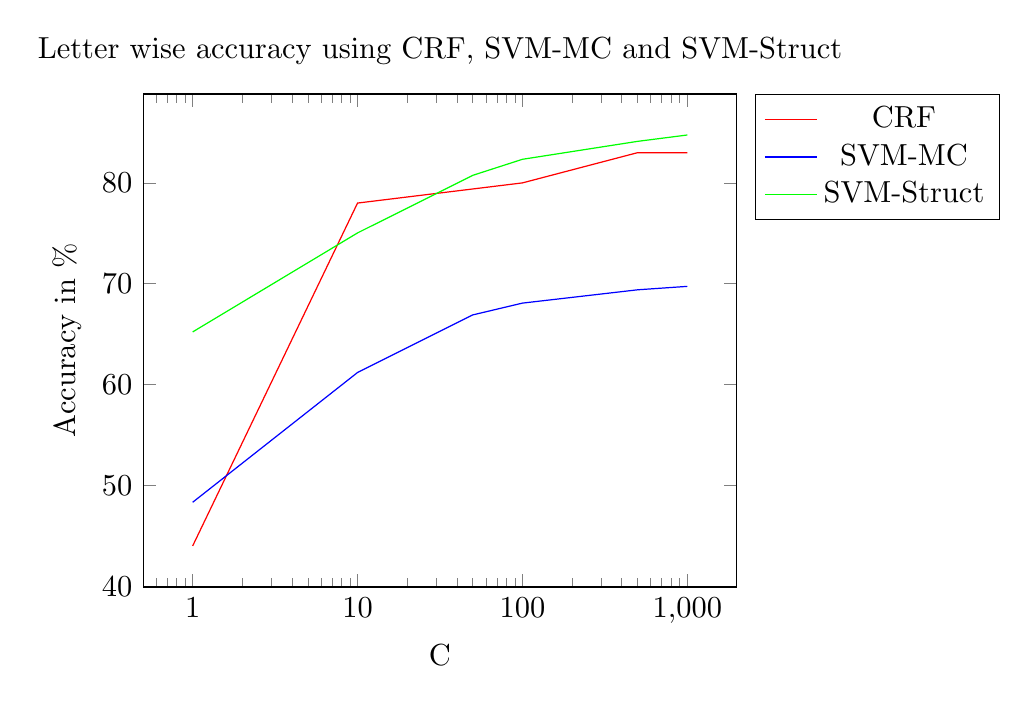
\begin{tikzpicture}[scale=1.1]
	\begin{semilogxaxis}[
	    log ticks with fixed point,
	    title={Letter wise accuracy using CRF, SVM-MC and SVM-Struct},
		xlabel=C,
		ylabel=Accuracy in \%,
		legend pos=outer north east]
	\addplot[color=red] coordinates {
		(1, 44)
		(10, 78)
		(100, 80)
		(500, 83)
		(1000, 83)
	};
	\addplot[color=blue] coordinates {
		(1, 48.33)
		(10, 61.20)
		(50, 66.91)
		(100, 68.08)
		(500, 69.40)
		(1000, 69.74)
	};
	\addplot[color=green] coordinates {
		(1, 65.22)
		(10, 75.04)
		(50, 80.75)
		(100, 82.34)
		(500, 84.12)
		(1000, 84.75)
	};
	\legend{CRF,SVM-MC,SVM-Struct}
	\end{semilogxaxis}
\end{tikzpicture}
\par\end{center}
Observation: SVM-Struct performs slightly better than CRF, whereas SVM-MC performs poorly. SVM-Struct performs better as it takes into consideration how much we dislike between the predicted and true output and as expected SVM-MC won't perform better as it takes into consideration only individual letters and not it's neighbourhood. 

\subsection{Accuracy on word wise prediction}

\begin{center}
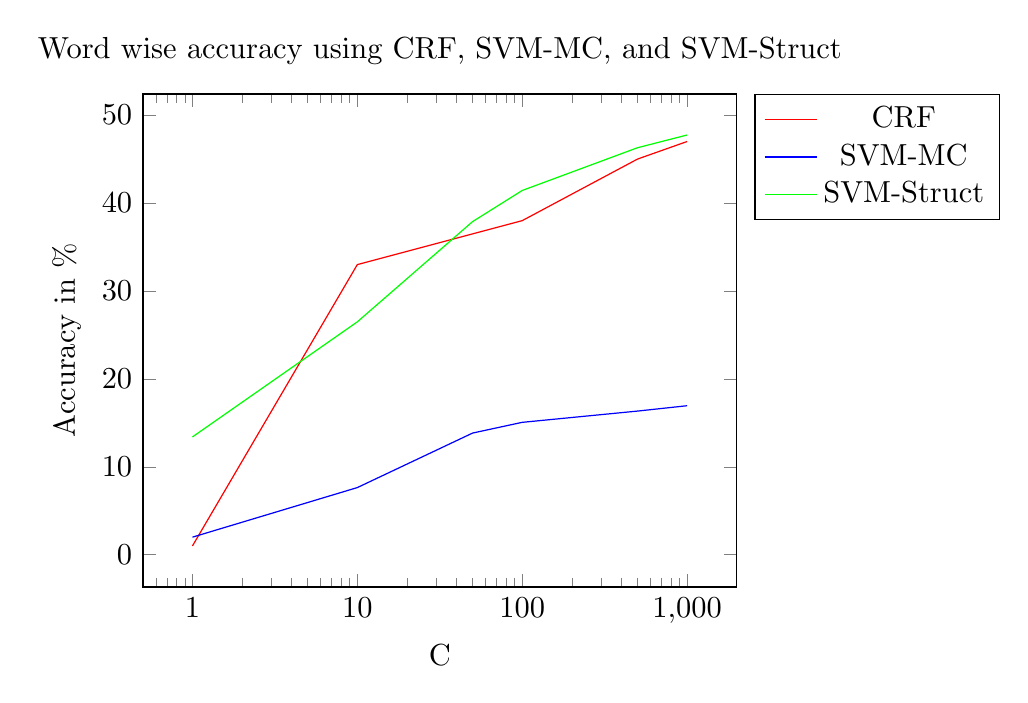
\begin{tikzpicture}[scale=1.1]
	\begin{semilogxaxis}[
	    log ticks with fixed point,
	    title={Word wise accuracy using CRF, SVM-MC, and SVM-Struct},
		xlabel=C,
		ylabel=Accuracy in \%,
		legend pos=outer north east]
	\addplot[color=red] coordinates {
		(1, 1)
		(10, 33)
		(100, 38)
		(500, 45)
		(1000, 47)
	};
	\addplot[color=blue] coordinates {
		(1, 2.00)
		(10, 7.64)
		(50, 13.84)
		(100, 15.06)
		(500, 16.34)
		(1000, 16.95)
	};
	\addplot[color=green] coordinates {
		(1, 13.40)
		(10, 26.49)
		(50, 37.889)
		(100, 41.43)
		(500, 46.29)
		(1000, 47.74)
	};
	\legend{CRF,SVM-MC,SVM-Struct}
	\end{semilogxaxis}
\end{tikzpicture}
\par\end{center}
Observation:
Again SVM-Struct and CRF outperforms SVM-MC and SVM-Struct performs slightly better than CRF due to the same above mentioned reasons and as we increase C the accuracy increases as we are able to fit our data more and more.

\section{Robustness to Tampering}
\subsection{Accuracy on letter wise prediction}

\begin{center}
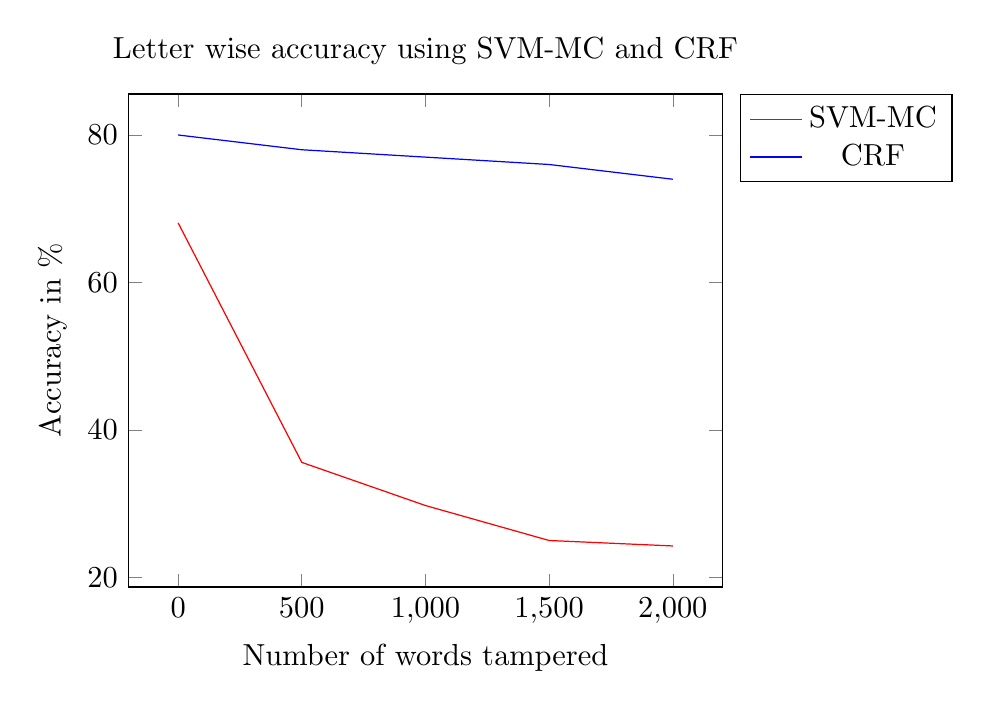
\begin{tikzpicture}[scale=1.1]
	\begin{axis}[
	    title=Letter wise accuracy using SVM-MC and CRF,
		xlabel=Number of words tampered,
		ylabel=Accuracy in \%,
		legend pos=outer north east]
	\addplot[color=red] coordinates {
		(0, 68.08)
		(500, 35.61)
		(1000,29.76)
		(1500, 25.02)
		(2000, 24.28)
	};
	\addplot[color=blue] coordinates 
	{
	    (0, 80)
		(500, 78)
		(1000,77)
		(1500,76)
		(2000,74)
	};
	\legend{SVM-MC,CRF}
	\end{axis}
\end{tikzpicture}
\par\end{center}
Observation:
CRF does much better than SVM-MC even when letters are tampered and the accuracy for CRF is more than 70\% which is more than 2 times the accuracy for SVM-MC. This shows the advantages of using CRF over SVM-MC as it takes into context of its neighbours.

\subsection{Accuracy on word wise prediction}

\begin{center}
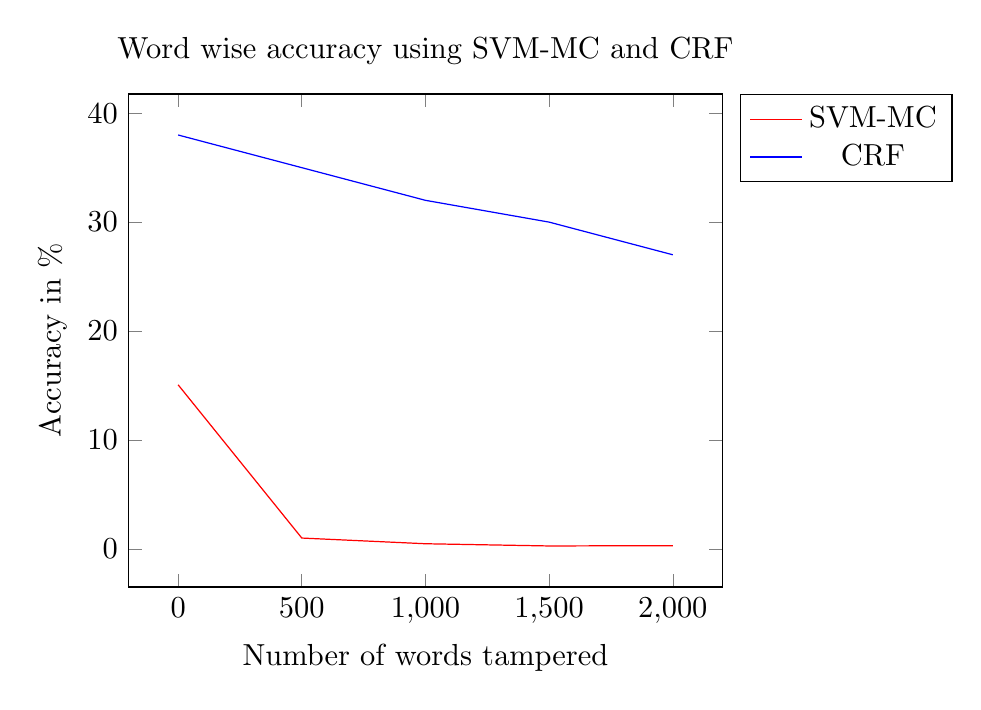
\begin{tikzpicture}[scale=1.1]
	\begin{axis}[
	    title=Word wise accuracy using SVM-MC and CRF,
		xlabel=Number of words tampered,
		ylabel=Accuracy in \%,
		legend pos=outer north east]
	\addplot[color=red] coordinates 
	{
		(0, 15.06)
		(500, 0.988)
		(1000,0.4652)
		(1500,0.2617)
		(2000,0.2907)
	};
	\addplot[color=blue] coordinates 
	{
	    (0, 38)
		(500, 35)
		(1000,32)
		(1500,30)
		(2000,27)
	};
	\legend{SVM-MC,CRF}
	\end{axis}
\end{tikzpicture}
\par\end{center}
Observation: Again CRF gives us a better result than SVM-MC as it takes into context of its neighbours and above all even when words are tampered the accuracy drops only slightly. On the other hand, SVM-MC does poorly as it doesn't take into context of its neighbours and when tampered the SVM-MC's accuracy is below 1\% which is not at all satisfactory.
\end{document}